\documentclass{acm_proc_article-sp}

\usepackage[latin1]{inputenc}
\usepackage[T1]{fontenc}

\usepackage{epsfig}
\usepackage{flafter}
\usepackage{graphicx}
\usepackage{times}

\begin{document}
%
% --- Author Metadata here ---
%
% Conference info for people whose papers are in the proceedings:
%
%\conferenceinfo{EWAS 2006 -- Third European Workshop on Aspects in Software,
%August 31, 2006, Enschede, The Netherlands.}
%{Technical report IAI-TR-2006-6, ISSN 0944-8535,
%Institut f\"{u}r Informatik III, Universit\"{a}t Bonn, Bonn, Germany
%}
%
% Conference info for people whose papers are NOT in the proceedings:
%
\conferenceinfo{EWAS 2006 -- Third European Workshop on Aspects in Software.}
{August 31, 2006, Enschede, The Netherlands
}


%\setpagenumber{50}
%\CopyrightYear{2002} % Allows default copyright year (2002) to be over-ridden - IF NEED BE.
%\crdata{0-12345-67-8/90/01}  % Allows default copyright data (X-XXXXX-XX-X/XX/XX) to be over-ridden.
% --- End of Author Metadata ---

\title{GAP: Generic Aspects for PHP}
\date{27 June 2006}

\numberofauthors{2}
\author{
\alignauthor Sebastian Bergmann\\
       \affaddr{eZ systems AS}\\
       \affaddr{Kverndalsgate 8}\\
       \affaddr{Postboks 253}\\
       \affaddr{N-3701 Skien (Norway)}\\
       \email{sb@ez.no}
\alignauthor G{\"u}nter Kniesel\\
       \affaddr{Department of Computer Science III}\\
       \affaddr{University of Bonn}\\
       \affaddr{R{\"o}merstrasse 164}\\
       \affaddr{D-53117 Bonn (Germany)}
       \email{gk@cs.uni-bonn.de}
}

\maketitle

\begin{abstract}
In this paper, we explore how aspect-oriented programming can be
implemented for the PHP programming language. We start with an
overview of existing implementations, identifying their strengths
and weaknesses. We then introduce \emph{GAP}, our implementation
of aspect-oriented programming for PHP that uses dynamic weaving,
supports aspect genericity, and provides a framework to implement
custom pointcut languages on top of it. The sum of these features
has previously been supported only in experimental research
prototypes that have had little impact on commercial software
development. In contrast, PHP has a large user community. In the
last decade, it has developed from a niche language for adding
dynamic functionality to small websites to a powerful tool making
strong inroads into large-scale, business-critical Web systems.
We expect that GAP will significantly ease development of such
systems while promoting a seamless integration of many advanced
concepts of aspect-oriented systems: aspect genericity, dynamic
weaving, a state-sensitive pointcut language, and extensibility.
\end{abstract}

\category{D.3.3}{Language Constructs and Features}{Abstract Data
Types} \terms{Design, Languages} \keywords{Generic Aspects, Dynamic
Weaving, PHP, Extensible Pointcut Language}

\section{Introduction}

PHP \cite{PHP} is a widely-used scripting language. Initially
designed for Web programming, it has developed to a
general-purpose object-oriented language making strong inroads
into large-scale, business-critical Web systems. For instance,
financial institutions develop and maintain the BASEL II
\cite{BASELII} credit and insurance rating tools using PHP and
Yahoo runs all its business on PHP (except the core of the search
engine). As of version 5, released July 2004, the PHP language
features an object model that is similar to the ones of Java and
C\# and integrates ideas from other programming languages. The key
technical contributor to PHP's success is its sim\-pli\-city,
which translates into shorter development cycles, easier
maintenance, and lower training costs. The second one is social --
the very large and vibrant community around it, which develops not
only PHP itself but also thousands of open source applications
that can be used off-the-shelf or as references for new
applications.

Given the wide-spread use and impact of PHP on current
web-centered software development, the benefits of a well-designed
integration of aspect-oriented programming in PHP would be huge.
However, existing attempts to support aspect-oriented programming
in PHP do not take advantage of the dynamic nature of the
language, ignore new aspect-oriented language concepts, such as
genericity, or are not compatible with new versions of the
language (see Section \ref{sec:stateOfArt}).

In this paper we present an approach that provides dynamicity and
compatibility to the official PHP language releases while
supporting a powerful aspect language model, including aspect
genericity. It is called \emph{GAP}, \textbf{G}eneric
\textbf{A}spects for \textbf{P}HP. A predecessor was presented in
\cite{sb06} under the name \emph{AspectPHP}. We have chosen to rename
our approach to GAP in order to avoid confusion with the
\emph{aspectPHP} project \cite{aspectPHP} and to emphasize the
support for aspect genericity.

\section{The State of AOP for PHP}\label{sec:stateOfArt}%
In this section, we give an overview of the different options for
implementing an aspect-oriented extension of PHP and review
existing implementations.

\subsection{Preprocessor}
A preprocessor can be used to perform source code transformations and
statically weave the aspect code into the base program. The result of this
weaving is PHP source code that can then be deployed in a standard PHP
environment.

\textbf{Existing Implementations. } %\\
\emph{PHPAspect} \cite{PHPAspect} extends the PHP language with
keywords inspired by AspectJ \cite{gk01}. Figure \ref{Singleton}
shows an implementation of the \emph{Singleton} design pattern
\cite{gof95} in PHPAspect. \emph{Aspect-Oriented PHP} \cite{AOPHP}
is largely similar to \emph{PHPAspect}, the main difference being
that the AOPHP compiler is implemented in Java.

\emph{PHPAspect} provides a compiler, written in PHP, that
performs static weaving using source code transformations (see
Figure \ref{PHPAspect}). PHPAspect is currently being
reimplemented in C, using an XML representation for the abstract
syntax trees and using XSLT for the weaving process (see figure
\ref{PHPAspect2}). With the use of XSLT and XPath the author of
\emph{PHPAspect} hopes to achieve independence for the lexical and
syntax analysis from the PHP version and more flexibility with
regard to the aspect language.

\begin{figure}[hbt]
\centering \small{\begin{verbatim}
<?php aspect Singleton {
  public $instances = array();

  pointcut singleton:new(*(*));

  around singleton {
    $i = $thisJoinPoint->getClassName();

    if (!isset($singleton->instances[$i])) {
      $singleton->instances[$i] = proceed();
    }

    return $singleton->instances[$i];
  }
}
?>
\end{verbatim}}
\caption{Singleton implementation in PHPAspect. PHP identifiers
prefixed with a \$ sign represent variables. The right arrow ->
represents field access or method invocation.} \label{Singleton}
\end{figure}

\begin{figure}
\centering
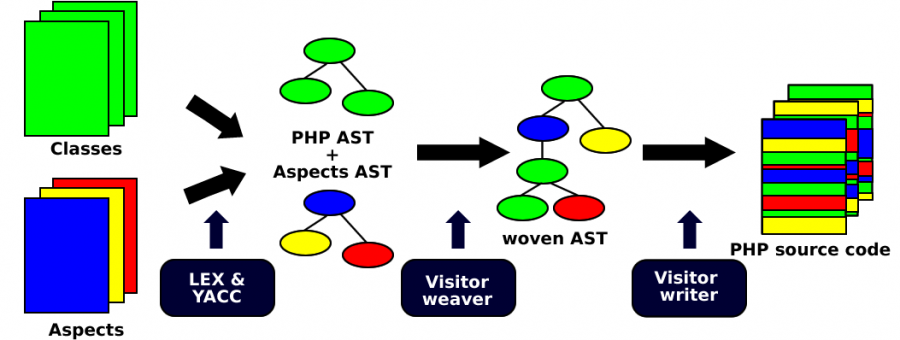
\includegraphics[width=8cm]{phpaspect_weaving}
\caption{The weaving chain of PHPAspect (from phpaspect.org)}
\label{PHPAspect}
\end{figure}

\begin{figure}[h!]
\centering
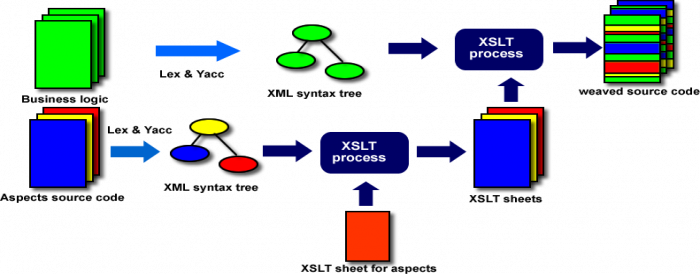
\includegraphics[width=8cm]{phpaspect_weaving2}
\caption{The new weaving chain of PHPAspect  (from phpaspect.org)}
\label{PHPAspect2}
\end{figure}

\textbf{Evaluation.} Since PHP is an interpreted, dynamic
language, static weaving comes with both advantages and
disadvantages. On the one hand, weaving is performed once before
deployment and has no performance impact at run-time. On the other
hand, static weaving imposes limits to both join point model and
pointcut language with regard to leveraging the dynamic nature of
the underlying programming language.

\subsection{Aspect-Aware PHP Interpreter}
Extensibility is one of the reasons why PHP became the favourite
"glue" of the Web. Functionality from existing third-party
libraries (database clients or image manipulation toolkits, for
instance) can be made available through PHP with the ease of use
one expects from a scripting language.

The \emph{Zend Engine}, the compiling and executing core of the
PHP Interpreter, can be extended using the C programming language.
An extension can be implemented either as a plug-in that can be
dynamically loaded or by changing the interpreter's source code.

\textbf{Evaluation.} % \\
Source changes enable changing or extending the language syntax by
modifying the scanner and parser rules. The resulting language
extension can only be distributed in the form of a custom binary
or a patch against the original source code of a specific version
of PHP. In contrast, a plug-in is developed using the public APIs
of the PHP interpreter and can therefore be deployed with
different versions of the language. For portability, a
plugin-based extension is preferable.

\textbf{Existing Implementations.} % \\
The \emph{aspectPHP} prototype \cite{aspectPHP} is a
reimplementation of Aspect-Oriented PHP \cite{AOPHP} in C. It is
available only as a patch for PHP 4.3.10, tying it closely to this
(meanwhile outdated) implementation of the language.

\subsection{Meta-Programming}
A language extension can be implemented in the PHP programming
language itself, using its meta-programming capabilities. These
include
\begin{itemize}
    \item \emph{a Reflection API} \cite{PHP-REFLECTION} for introspecting
          at runtime classes, methods, etc.
    \item \emph{interceptor methods} inspired by the
\texttt{doesNotUnderstand} selector of Smalltalk \cite{mw87}. In
PHP, read and write access to undeclared attributes and calls to
undeclared methods of an object are handled by the methods
\texttt{\_\_get()}, \texttt{\_\_set()}, and \texttt{\_\_call()}.
    \item \emph{byte code modification} via the Runkit extension
    \cite{RUNKIT}.
\end{itemize}

\textbf{Existing Implementations. } %\\
The \emph{AOP Library for PHP} \cite{AOPL4PHP} is a PHP library
that supports just a very rudimentary join point model and
requires extensive manual changes to the base code, failing to
support the two main characteristics of aspect-oriented systems:
obliviousness and quantification \cite{filman00}.

\begin{figure}[h!]%
\centering \small{\begin{verbatim}

<?php
require_once 'AClass.php';
require_once 'aop.lib.php';

$aspect   = new Aspect;
$pointCut = $aspect->pointcut('call AClass::aMethod');
$pointCut->_before('... before advice code ...');
$pointCut->_after('... after advice code ...');
$pointCut->destroy();

$object = new AClass($aspect);
?>

<?php class AClass {
    private $aspect;

    public function __construct($aspect) {
        $this->aspect = $aspect;
    }

    public function aMethod() {
        Advice::_before($this->aspect);
        // ... base code ...
        Advice::_after($this->aspect);
    }
} }?>
\end{verbatim}}
\caption{Aspect declaration with the AOP Library for PHP and base
class using the aspect. The ``aspect'' is just a library that is
invoked explicitly from the base code.} \label{AOPL4PHP-Aspect}
\end{figure}

Figure \ref{AOPL4PHP-Aspect} shows how to declare ``aspects'' and
advice using the AOP Library for PHP such that invocation of
\texttt{aMethod()} in \texttt{AClass()} invokes first the
\texttt{before} advice code, then the base code of the method, and
finally the \texttt{after} advice code. The example illustrates
that the base code has to be modified extensively for using the
aspect. First, the constructor of the base class needs to be
changed to accept an \texttt{\$aspect} object and store it in an
instance variable\footnote{
%
\texttt{\_\_construct()} is the name of the constructor method in
PHP.
}. %
Then, explicit calls to this object's \texttt{\_before()} and
\texttt{\_after()} methods have to be inserted to each method of
the class. This is not different from any other invocation of
library code. Therefore the claim of supporting AOP is hardly
justified.

\textbf{Evaluation.} Whereas the only existing attempt to bring
aspects to PHP using its metalevel features can hardly be
recommended, the metaprogramming approach cannot be dismissed in
general. On the contrary, it has the potential to take advantage
of PHP's dynamicity and to provide a portable solution, that is
compatible with different language versions.

\subsection{State of Art Summary}
Our short review has shown that from the four attempts to bring
aspect-oriented concepts to PHP only three really provide
aspect-oriented functionality. Of these, one is hard-coupled to an
outdated language version. The other two are based on static
weaving, falling short of leveraging on the dynamic language
features of PHP in aspects. In addition, they are based on the
language model of AspectJ, which does not support some powerful
new concepts that are particularly well-suited for the development
of large web-based applications: genericity, and a state-aware,
extensible pointcut language. %, and dynamic weaving.

\section{GAP: Generic Aspects for PHP}
In this section we introduce \emph{GAP}, our implementation of
aspect-oriented programming for PHP. GAP supports an extensible
pointcut language, aspect genericity, and dynamic weaving. Taking
advantage of PHP's meta-programming capabilities, this is achieved
without changing the language syntax or interpreter.

% /* Additionally, GAP leverages on the dynamic nature of PHP by
% offering a state-aware join point model. <-- *** Das sollten
% wir wieder einf{\"u}gen, wenn es tats{\"a}chlich soweit ist.
% */

\subsection{Aspect Basics}

In GAP aspects are plain PHP classes that use annotations in
comments to declare pointcuts, advice, and inter-type
declarations. Advice declarations bind a pointcut expression to an
invocation of a plain PHP method that takes a join point object as
parameter. The method implements the advice body. It will be
executed on all join points matching the pointcut expression.

In GAP, custom pointcuts can be implemented easily based on an
open pointcut language framework (see section
\ref{OpenArchitecture}). In its standard configuration GAP allows
quantifications over three join point types:
\begin{itemize}
  \item Object initialization
  \item Field access
  \item Method call or execution
\end{itemize}


\begin{figure}[thb]
\centering \small{%
\begin{verbatim}
<?php
/* @pointcut allInvocations : method(* *->*(..));
 * @after    allInvocations : Logging->log();
 */
class Logging {
  public function log($joinPoint) {
    printf(
      "%s->%s() called %s->%s()\n",
      $joinPoint->getSource()
                ->getDeclaringClass()
                ->getName(),
      $joinPoint->getSource()
                ->getName(),
      $joinPoint->getTarget()
                ->getDeclaringClass()
                ->getName(),
      $joinPoint->getTarget()
                ->getName()
    );
  }
} ?>
\end{verbatim}}
\caption{GAP aspect that logs all method calls}
\label{LoggingAspect}
\end{figure}

The currently implemented pointcut syntax is similar to the one of
AspectJ (see Figure \ref{tab:pointcuts}).
For instance, the first line of the comment in Figure
\ref{LoggingAspect} declares a pointcut that matches all method
invocations. The \texttt{@pointcut allInvocations} annotation
starts the declaration of a pointcut named
\texttt{allInvoca\-tions}. The \texttt{method} keyword is the
selector for the combined \emph{Method Call} / \emph{Method
Execution} join point in GAP's join point model. The pattern
\texttt{* *->*(..)} matches methods with arbitrary visibility
(first star), class name (second star), method name (third star),
and parameter list (double dots).

\begin{table}[b!]
\begin{tabular}{l}
  \hline
  % after \\: \hline or \cline{col1-col2} \cline{col3-col4} ...
  \textbf{Predefined GAP Pointcuts}\\
  \hline
  \small{\texttt{initialization(\emph{class}(\emph{parameters}))}}\\
  \small{\texttt{get(\emph{modifier} \emph{class}->\emph{attribute})}} \\
  \small{\texttt{set(\emph{modifier} \emph{class}->\emph{attribute})}}\\
  \small{\texttt{method(\emph{modifier} \emph{class}->\emph{method}(\emph{parameters}))}}\\
  \small{\texttt{source(\emph{modifier} \emph{class}->\emph{method}(\emph{parameters}))}}\\
  \small{\texttt{cflow(\emph{modifier} \emph{class}->\emph{method}(\emph{parameters}))}}\\
  \hline
\end{tabular}
\caption{Implemented pointcuts demonstrating the versatility of
GAP's extensible pointcut framework. Italics indicate
non-terminals} \label{tab:pointcuts}
\end{table}

Note that the \texttt{allInvocations} pointcut from Figure
\ref{LoggingAspect} also matches the execution of the
\texttt{log()} advice method. However, invoking an advice method
for the execution of an advice method is currently disabled in GAP
in order to avoid certain sources of aspect interference. Whether
this is too restrictive could be a topic of discussion at the
workshop.

Join points are represented by \texttt{GAP\_JoinPoint} instances.
For each kind of join point supported by GAP's join point model
there is a specific implementation of \texttt{GAP\_JoinPoint}. For
instance, the class \texttt{GAP\_JoinPoint\_MethodCall} implements
GAP's combined method call and method execution join point. Its
instances include information on the calling object, the calling
method, the called object, and the called method. This information
is represented by objects from the Reflection API, in this case
two instances of the \texttt{ReflectionMethod} class, representing
the caller and callee, respectively.

Through the information provided by the \texttt{\$joinPoint} an
advice method that is invoked for a method execution join point
can find out which method called the method associated with the
current join point. This information is also used by the
additional pointcut expressions supported by GAP's prepackaged
pointcut language implementation: source and cflow (see Table \ref{tab:pointcuts}).
%
%\begin{itemize}
%\small{
%  \item \texttt{source(<modifier> <class>-><method>(<parameters>))}
%  \item \texttt{cflow(<modifier> <class>-><method>(<parameters>))}
%}
%\end{itemize}
%
The \texttt{source()} pointcut expression matches the immediate
method that performed an object instantiation, attribute access,
or method call. The \texttt{cflow()} pointcut expressions matches
if the specified method is on the current call stack.

Pointcuts can be associated with the following aspect effects
\cite{kr06}:

\begin{itemize}
    \item \emph{Advice}: Execution of code before, after or around
          any of the above-mentioned join points (indicated by the
          annotations \texttt{@before}, \texttt{@after}, or
          \texttt{@around}).
    \item \emph{Declarations}: Addition and change of fields, methods,
          inheritance relations and interface implementation declarations
          (indicated by the keyword \texttt{@introduce}).
    \item \emph{Custom Errors}: With the \texttt{declare error} or
          \texttt{declare warning} syntax one can customize the
          response to the occurrence of a join point, as shown in
          Figure \ref{fig:FactoryEnforcement}.
\end{itemize}

The second line of the comment in Figure \ref{LoggingAspect} shows
a GAP advice. The \texttt{@after} annotation binds the method
\texttt{log} of class \texttt{Logging} to the previously defined
pointcut \texttt{allInvocations}. The overall effect of Figure
\ref{LoggingAspect} is the declaration of an aspect named
\texttt{Logging} that invokes the advice named \texttt{log()}
after every method call. The join point context is passed to the advice
method as an object of the type \texttt{GAP\_JoinPoint}.

\begin{figure}[t]
\centering \small{
\begin{verbatim}
<?php
/**
 * @pointcut inFactory : method(Factory->get(..));
 * @pointcut newObject : initialization(Base+(..));
 * @declare error : !inFactory && newObject
 *                : "Factory::get() must be used.";
 */
class Factory {
    public static function get($type)
    {
        return new $type;
    }
}
?>
\end{verbatim}}
\caption{GAP aspect that enforces the use of a Factory method}
\label{fig:FactoryEnforcement}
\end{figure}

\subsection{Aspect Genericity}
The implementations of aspect-oriented programming for PHP that we
discussed in Section \ref{sec:stateOfArt} introduce strong
dependencies of aspects on base code by requiring aspects to use
concrete names of types, classes, methods, and other entities from
base programs.

Wildcards, such as \texttt{*} and \texttt{..} are intended to alleviate this
problem but are no real solution since they throw the child out with the bath.
Instead of being too specific, they are too general. They match more than
intended because it is not possible to express dependencies of the values
matched by different wildcards.

As a solution to this problem, generic aspect languages
\cite{kr06} such as LogicAJ \cite{windeln03}, Sally \cite{sh03},
Carma \cite{kg03}, and OReA \cite{mdh04} replace wildcards (e.g.
\texttt{*}) by named logic meta-variables (e.g. \texttt{?var}).
All occurrences of \texttt{?var} in a pointcut expression must match
the same value. Further constraints on the legal matches can be expressed
by additional predicates that can be used in pointcut definitions. The
\texttt{source} predicate used in Figure \ref{fig:LoggingAspect-MetaVariables}
is an example. It does not select join points but only constrains the
matches of the \texttt{method} predicate.

Figure \ref{fig:LoggingAspect-MetaVariables} shows how GAP supports
meta-variables in its annotation-based pointcut language. The
\texttt{localCalls} pointcut captures all method invocations that
address methods from the same class. The values of meta-variables that
matched during the evaluation of the pointcut expression can be accessed
via the \texttt{\$joinPoint} object's \texttt{getMetaVariable} method.

\begin{figure}[t]
\centering
\small{
\begin{verbatim}
<?php
/* @pointcut localCalls : method(* ?class->*(..))
 *                     && source(* ?class->*(..));
 * @after    localCalls : Logging->log();
 */
class Logging {
  public function log($joinPoint) {
    printf(
      "%s::%s() called %s::%s()\n",
      $joinPoint->getMetaVariable('class'),
      $joinPoint->getSource()->getName(),
      $joinPoint->getMetaVariable('class'),
      $joinPoint->getTarget()->getName()
    );
  }
}
?>
\end{verbatim}}
\caption{GAP aspect using a pointcut with meta-variables
 to express logging of \emph{local} calls}
\label{fig:LoggingAspect-MetaVariables}
\end{figure}

\section{Implementation of GAP}
In this section we show how we implemented GAP in PHP using only
its Reflection API, interceptor methods and the Runkit extension.

\subsection{Open Architecture}
\label{OpenArchitecture} The two main components of the GAP plugin
are the \texttt{GAP\_Weaver} class and the
\texttt{GAP\_Dispatcher} class. They are the core of GAP on top of
which the join point model and pointcut language framework are
built. The latter provides the building blocks for implementing a
pointcut language. Figure \ref{POINTCUT-FRAMEWORK} shows a subset
of these building blocks. Together with the \emph{pointcut
registry} they provide a way to capture join points and activate
advice code. However, this low-level declaration of join points
and advice is not convenient and practical for everyday use.
Therefore, these internals of the API are hidden behind the
annotation-based pointcut and advice declaration syntax introduced
in the previous section. Using the basic classes, other
implementors can extend the pointcut language with new built-in
pointcut definitions.

\begin{figure}%
\centering
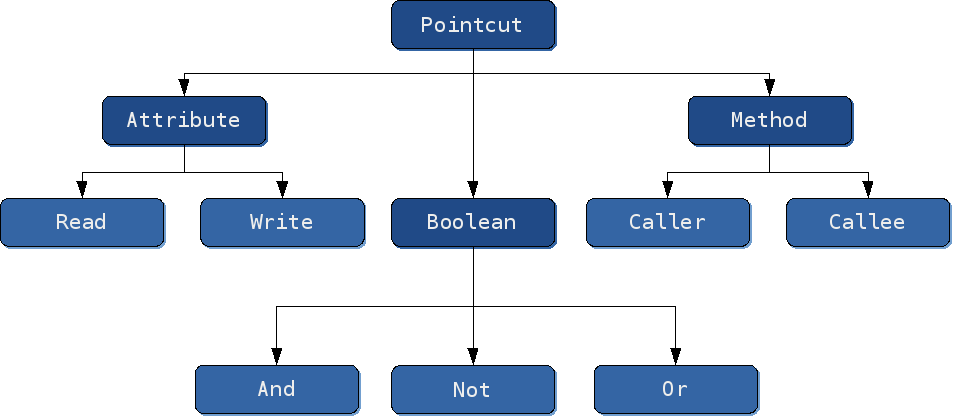
\includegraphics[width=8cm]{gap_pointcut_framework}
\caption{Subset of the GAP Pointcut Framework}
\label{POINTCUT-FRAMEWORK}
\end{figure}

\begin{figure*}%
\centering
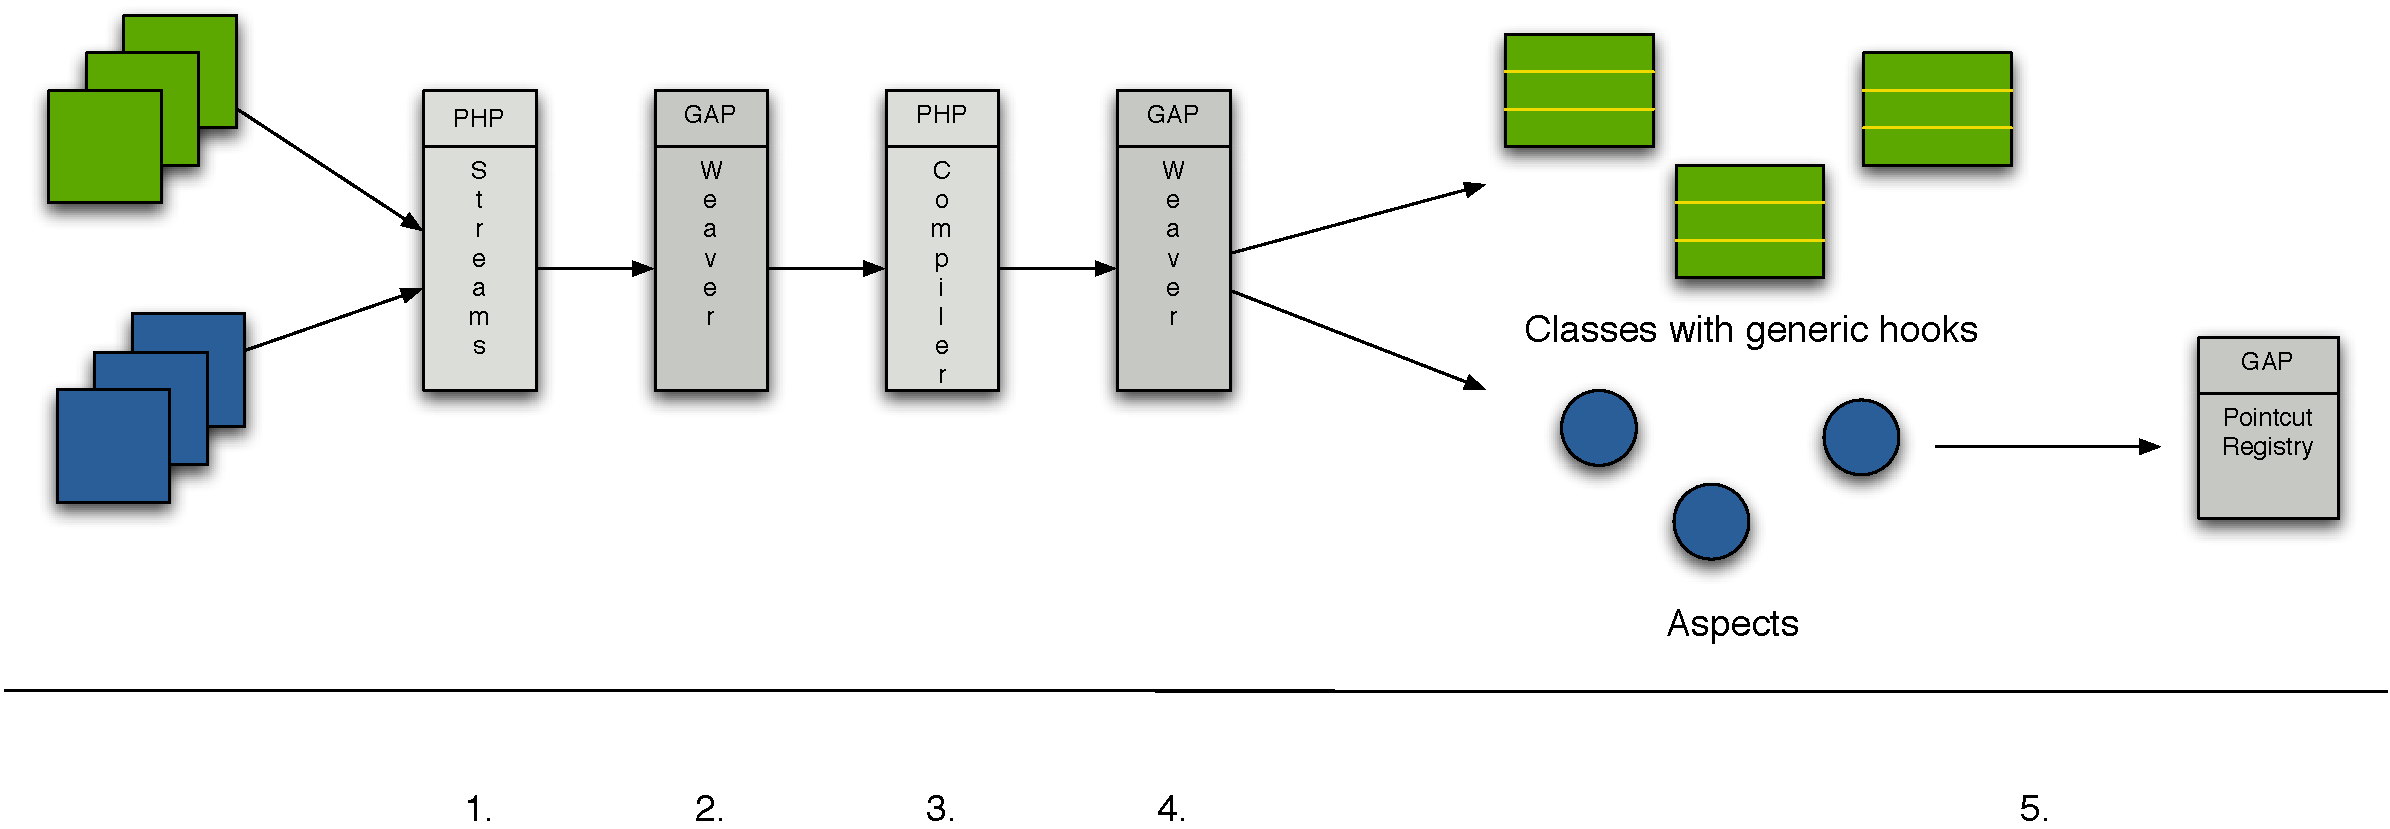
\includegraphics[width=15.5cm]{gap_weaving.pdf}
\caption{The weaving chain of GAP} \label{fig:GAP-Weaver}
\end{figure*}

\subsection{Load-Time Hooks for Dynamic Weaving}
The PHP Interpreter uses its \emph{Streams Layer}
\cite{PHP-STREAMS} to load PHP source files. This layer provides a
unified approach to the handling of files and sockets. Any stream,
once opened, can also have any number of \emph{filters} applied to
it, which process data as it is read from or written to the
stream.

Figure \ref{fig:GAP-Weaver} illustrates the GAP weaving chain:
Using a streams filter written in PHP, the GAP Weaver hooks into
the loading of the source code of classes (green) and aspects
(blue). The first weaving stage performs source code
transformations and passes the modified source code to the
compiler integrated in the PHP Interpreter. The second weaving
stage operates on the bytecode generated by the compiler and uses
the Runkit extension to complete the insertion of generic hooks
into the classes. The pointcut expressions of the aspects are
evaluated and stored in the \emph{Pointcut Registry} that is used
by the \emph{GAP Dispatcher} to capture join point events at
run-time and dispatch the appropriate advices. The actual advice
execution can be dynamically turned off at runtime.

GAP's annotation-based declaration of pointcuts and advice is
implemented as follows:
\begin{itemize}
\item When loading the source code for an aspect, the class
      representing the aspect is searched for annotations,
      using the Reflection API of PHP. The annotations are
      parsed and converted into an object representation.
      For instance, the \texttt{@pointcut} annotation,
      is parsed into a tree of \texttt{GAP\_Pointcut}
      objects that is then passed to the Pointcut Registry.
      Similarly, the associations of pointcuts and
      advice is parsed and registered.
\item When loading the source code for a class, the appropriate
      inter-type declarations are inserted into the bytecode of
      the class and the generic hooks for advice execution are
      inserted into the bytecode of its methods. Byte code
      manipulation is performed using the Runkit extension
      of the PHP Interpreter.
\end{itemize}

In the remainder of this section we explain how the generic hooks
for the three different join point types are implemented in
detail.

\textbf{Method Call Hook} Each method of the processed class is
replaced by a proxy method that calls the \texttt{methodCall()}
method of the \texttt{GAP\_Dispatcher} class. This method has
access to the original implementation of the proxy method
and can execute it between the execution of before- and
after-advices. Figure \ref{weaveMethodJoinPoint} shows
the PHP implementation of this scheme.

\textbf{Attribute Access Hook} Each attribute of the class is
renamed so that accessing it using the original name triggers a
call to the \texttt{\_\_get()} (for read access) or
\texttt{\_\_set()} (for write access) method. Implementations of
these interceptor methods  are woven into the class, too. They
call the \texttt{attributeRead()} and \texttt{attributeWrite()}
methods of the \texttt{GAP\_Dispatcher} class.

\textbf{New Object Hook.} The weaving of the hook for capturing
the \emph{New Object} join point is an exception from the abobe
scheme, as it is actually performed on the source code level. It
replaces calls to the \texttt{new} operator with corresponding
calls to the \texttt{newObject()} method of the
\texttt{GAP\_Dispatcher} class.

\subsection{Run-Time Dispatcher}
During program execution, the previously introduced hooks for the
join points check whether or not an the pointcut registry contains
a pointcut that matches the current join point. If that is the
case, the \texttt{GAP\_Dispatcher} class handles the execution of
the corresponding advice and passes the current context in the
form of an \texttt{GAP\_JoinPoint} object to the advice method.

%The implementation of this scheme for method call join points is
%shown in Figure \ref{methodCall}. The methods \texttt{methodCallBefore()} and
%\texttt{methodCallAfter()} check, based upon the information
%contained in the \texttt{\$joinPoint} object, whether a registered
%pointcut matches the current join point and dispatch the advice
%execution accordingly.
%
%The \texttt{\$joinPoint} object is built using the
%\texttt{debug\_backtrace()} function \cite{PHP-DEBUG-BACKTRACE}
%that is provided by PHP. This function allows read access to the
%current callstack and returns it in the form of an associative
%array. For each method call that is currently on the call stack,
%this array contains an entry with a reference to the calling object,
%the name of the calling method, as well as the arguments passed to
%the method.

\begin{figure}[thb]%
\centering{
\small{
\begin{verbatim}
protected static function weaveMethodJoinPoint(
    ReflectionMethod $method
) {
  runkit_method_rename(
    $method->getDeclaringClass()->getName(),
    $method->getName(),
    '__GAP_' . $method->getName()
  );

  runkit_method_add(
    $method->getDeclaringClass()->getName(),
    $method->getName(),
    self::generateMethodParameters($method),
    'return GAP_Dispatcher::getInstance()->
     methodCall('.
    '  new GAP_JoinPoint_Method'.
    ');'
  );
}
\end{verbatim}}}
\caption{The GAP\_Weaver::weaveMethodJoinPoint() method}
\label{weaveMethodJoinPoint}
\end{figure}

%\begin{figure}%[hbt]
%\centering\small%
%{\begin{verbatim}
%public function methodCall(
%       GAP_JoinPoint_Method $joinPoint
%) {
%    // Invoke before-advice.
%    $this->methodCallBefore($joinPoint);
%
%    // Check whether the method call
%    // should be performed.
%    // A caching advice, for instance,
%    // can prevent the execution of the
%    // captured method call.
%    if ($joinPoint->shouldExecute()) {
%        // Perform the captured method call
%        // and store the result in the
%        // $joinPoint object for later access
%        // by the after-advice.
%        $joinPoint->setReturnValue(
%          $joinPoint->target->invoke(
%            $joinPoint->targetObject,
%            $joinPoint->getArguments()
%          )
%        );
%    }
%
%    // Invoke after-advice.
%    return $this->methodCallAfter($joinPoint);
%}
%\end{verbatim}}
%\caption{The GAP\_Dispatcher::methodCall() method} \label{methodCall}
%\end{figure}

\subsection{Evaluation}
The flexibility of dynamic weaving comes at the price of a
possible performance hit. For every execution, for instance, a
request to a PHP-driven website, the aspect code has to be woven
into the base program. During the execution of the program there
are two additional method calls for every attribute access, method
call (see figure \ref{GAP-Dispatcher}), and execution of the
\texttt{new} operator. Run-time measurements and performance
comparisons with other implementation schemes are still to be
carried out.

\begin{figure}[hbt]
\centering
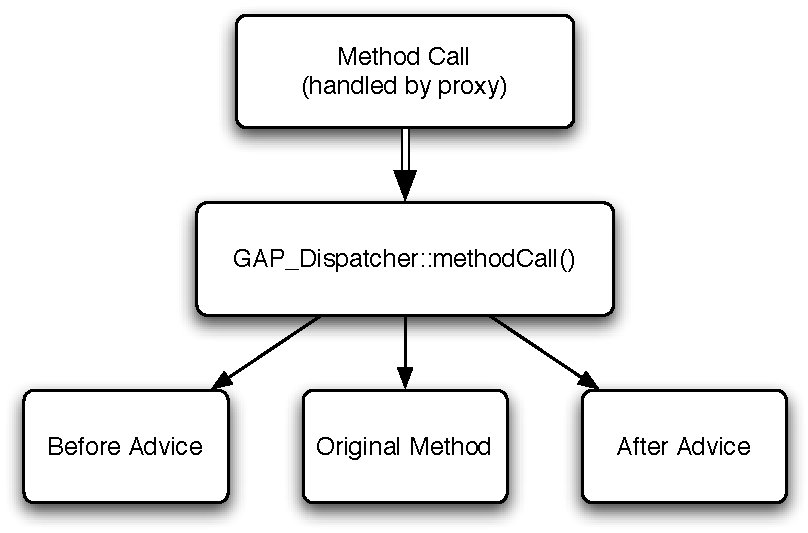
\includegraphics[width=8cm]{gap_dispatcher.pdf}
\caption{Dispatching Method Call Advices} \label{GAP-Dispatcher}
\end{figure}

\section{Related Work}

This paper presented GAP, an extension of the PHP programming
language with aspect-oriented programming concepts. Compared to
other implementations of aspect-oriented programming for PHP (see
Section \ref{sec:stateOfArt}) GAP stands out as being the first
implementation that supports dynamic weaving, genericity, and an
extensible pointcut language.

Compared to non-PHP aspect languages and systems, GAP provides a
specific mix of partly well-known concepts and techniques. GAP's
design balances the expressive power of generic aspect languages
such as LogicAJ \cite{windeln03}, Sally \cite{sh03}, Carma
\cite{kg03} and OREA \cite{mdh04} with the simplicity of the
design of Classpects \cite{hrkjs05}. With the formers it shares
the concept of logic meta-variables. With the latter it shares the
reliance on plain base level methods as the body of advice.

The open architecture of GAP allows the implementation of
customized pointcut languages on top of a common kernel that
handles the weaving and dispatching of aspect code. In this
respect, GAP has similarities with various other systems built on
reflection and to open and extensible systems such as Josh \cite{sckn04}
and LogicAJ 2 \cite{trgkma06}.

Implementation-wise, GAP's dispatch mechanism is related to the
method wrappers of Brant, Foote, Johnson and Roberts, which are a
standard mechanism in Smalltalk implementations and the basis of
aspect-oriented extensions of Smalltalk, such as AspectS \cite{rh01}.
Load-time weaving of byte code is based on the filter concept of PHP
that provides the generic class file interception functionality that
has only recently been integrated into Java 5 (see
\texttt{java.lang.instrument}) and has previously required specific
solutions such as JMangler \cite{gkpcma04}.
Use of load time weaving as a way to implement generic hooks that
enable run-time weaving has been pioneered in JAC \cite{rp04}. The
pointcut registry and dispatcher mechanism are recurring themes in
various dynamic weaving systems and theoretical models of aspect
orientation. % (***references to dynamic weaving and theoretical models to be added***).

\section{Conclusions and Future Work}
This paper presented GAP, an extension of the PHP programming
language with aspect-oriented programming concepts. Compared to
other implementations of aspect-oriented programming for PHP GAP
stands out as being the first implementation that supports dynamic
weaving, genericity, and an extensible pointcut language.

Compared to other aspect languages and systems, GAP provides a
specific mix of partly well-known concepts and techniques. Its
specific power is the orthogonal integration of all these features
into a widely-used programming language. We hope that the use of
GAP as a powerful, dynamic extension to PHP will foster the
adoption of aspect-oriented technologies in a community that is
not using the research prototypes that have first demonstrated
some of the more advanced techniques (e.g. generic aspects).

As a long-time contributor to PHP the first author had early
access to new Runkit features that are still to be made available
publicly. Therefore, we will wait with the first public release of
GAP until they are available. We will use this time to further
improve GAP's pointcut language and performance.

The dynamic interpretation of the pointcut expressions at runtime
allows for state-sensitive pointcut languages. Possible
applications of state awareness includes the selective execution
of advice depending on information about the user that requests a
website document, his domain name or web browser, for instance. We
are still thinking about an elegant syntax to integrate support
for state sensitivity to our annotation-based pointcut language.

Further benchmarking will have to show whether or not the
deployment of GAP in the web-server environment that is usually
associated with PHP is practical in spite of the performance hit
incurred by the flexibility of dynamic weaving. The
\texttt{GAP\_Dispatcher} class could be implemented in C as an
extension to the PHP Interpreter to improve the run-time
performance.

Our incentive to develop GAP, however, was not primarily in using it in a
web-server environment but rather in the development of tools such
as \emph{PHPUnit} \cite{PHPUnit}. GAP could be used, for instance,
to implement Mock Objects through an aspect that implements class
posing (following \cite{kr06}[Figure 6]) or to enforce design constraints at development
time as illustrated in Figure \ref{fig:FactoryEnforcement}.
Another usage scenario for GAP lies within the PHP-GTK \cite{PHP-GTK}
environment, which provides an object-oriented interface to GTK+ \cite{GTK}
classes and functions and facilitates the writing of client-side
cross-platform GUI applications using PHP.

\section{Acknowledgements}
Sebastian Bergmann, who is a long-time contributor to the PHP
project, would like to thank his peers from the PHP community in
general and Sara Golemon, the author of the Runkit extension, in
particular. He is also thankful for the support and encouragement
from Prof. Dr. Armin B. Cremers, head of the Computer Science
Department III at the University of Bonn.

\bibliographystyle{abbrv}
\begin{thebibliography}{}

\bibitem{sb06}
Sebastian Bergmann. \emph{AspectPHP: An Aspect-Oriented Programming Extension for the PHP Programming Language},
Poster, In: Student Research Extravaganza. Poster Session of the Fifth International Conference on Aspect-Oriented Software Development (AOSD.06), 2006, Bonn.

\bibitem{gk01}
Gregor Kiczales, Erik Hilsdale, Jim Hugunin, Mik Kersten, Jeffrey Palm, William G. Griswold. \emph{An Overview of AspectJ}, In: Lecture Notes in Computer Science, volume 2072, pages 327-355, 2001.

\bibitem{gof95}
Erich Gamma, Richard Helm, Ralph Johnson, John Vlissides. \emph{Design Patterns: Elements of Reusable Object-Oriented Software}, Addison-Wesley, 1995.

\bibitem{mw87}
Mario Wolczko. \emph{Semantics of Smalltalk-80}, In: Proceedings of the 1987 European Conference on Object-Oriented Programming, J. B\'ezivin, J.-M. Hullot, P. Cointe, and H. Lieberman, editors, Lecture Notes in Computer Science, volume 276, pages 108-120. Springer-Verlag, Paris, June 1987.

\bibitem{filman00}
Robert E. Filman and Daniel P. Friedman. \emph{Aspect-Oriented Programming is Quantification and Obliviousness}, In: Workshop on Advanced Separation of Concerns, OOPSLA 2000, October 2000, Minneapolis.

\bibitem{kr06}
G{\"u}nter Kniesel, Tobias Rho. \emph{A Definition, Overview and Taxonomy of Generic Aspect Languages}, L'Objet, vol. 11, 3, pp. , to appear, Hermes Science, London.

\bibitem{windeln03}
Tobias Windeln. \emph{LogicAJ -- Eine Erweiterung von AspectJ um logische Meta-Programmierung} (in German), Diploma Thesis, CS Dept. III, University of Bonn, Germany, August 2003.

\bibitem{sh03}
Stefan Hanenberg, Rainer Unland. \emph{Parametric Introductions}, In: Proceedings of the 2nd International Conference on Aspect-Oriented Software Development (AOSD.03), 2003, Boston, MA.

\bibitem{kg03}
Kris Gybels, Johan Brichau. \emph{Arranging Language Features for More Robust Pattern-Based Crosscuts}, In: Proceedings of the 2nd International Conference on Aspect-Oriented Software Development (AOSD.03), 2003, Boston, MA.

\bibitem{mdh04}
Maja D'Hondt. \emph{Hybrid Aspects for Integrating Rule-Based Knowledge and Object-Oriented Functionality}, Ph.D. Thesis, Vrije Universiteit Brussel, May 2004.

\bibitem{hrkjs05}
Hridesh Rajan, Kevin J. Sullivan.\emph{Classpects: Unifying Aspect- and Object-Oriented Language Design}, In: Proceedings of the 27th International Conference on Software Engineering, 2005, St. Louis, MO.

\bibitem{sckn04}
Shigeru Chiba, Kiyoshi Nakagawa. \emph{Josh: An Open AspectJ-like Language}, In: Proceedings of the 3rd International Conference on Aspect-Oriented Software Development (AOSD.04), 2004, Lancaster, UK.

\bibitem{trgkma06}
Tobias Rho, G{\"u}nter Kniesel, Malte Appeltauer. \emph{Fine-Grained Generic Aspects}, In: Workshop on Foundations of Aspect-Oriented Languages (FOAL'06), in conjunction with the Fifth International Conference on Aspect-Oriented Software Development (AOSD.06), 2006, Bonn.

\bibitem{rh01}
Robert Hirschfeld. \emph{AspectS: AOP with Squeak}, In: OOPSLA'01 Workshop on Advanced Separation of Concerns, 2001, Tampa, FL.

\bibitem{gkpcma04}
G{\"u}nter Kniesel, Pascal Costanza, Michael Austermann. \emph{JMangler - A Powerful Back-End for Aspect-Oriented Programming}, In: Aspect-Oriented Software Development, Prentice Hall, 2004.

\bibitem{rp04}
R. Pawlak, L. Duchien, L. Seinturier, G. Florin, F. Legond, L. Martelli. \emph{JAC: A Framework for Separation of Concerns and Distribution}, In: Aspect-Oriented Software Development, Prentice Hall, 2004.

\bibitem{PHP}
http://www.php.net/

\bibitem{BASELII}
http://en.wikipedia.org/wiki/Basel\_ii

\bibitem{aspectPHP}
http://www.cs.toronto.edu/$\sim$yijun/aspectPHP/

\bibitem{PHPAspect}
http://www.phpaspect.org/

\bibitem{AOPHP}
http://www.aophp.net/

\bibitem{PHP-REFLECTION}
http://www.php.net/manual/en/language.oop5.reflection.php

\bibitem{RUNKIT}
http://www.php.net/runkit

\bibitem{AOPL4PHP}
http://www.phpclasses.org/aopinphp

\bibitem{PHP-STREAMS}
http://www.php.net/manual/en/streams.php

\bibitem{PHP-DEBUG-BACKTRACE}
http://www.php.net/debug\_backtrace

\bibitem{PHPUnit}
http://www.phpunit.de/

\bibitem{PHP-GTK}
http://gtk.php.net/

\bibitem{GTK}
http://www.gtk.org/

\end{thebibliography}

\end{document}
